\documentclass[journal, 12pt, twocolumn]{article}
\usepackage[utf8]{inputenc}
\usepackage{enumitem}
\usepackage{amsmath}
\usepackage{amssymb}
\usepackage{graphicx}
\graphicspath{ {./figure} }
\usepackage[export]{adjustbox}
\setlength{\columnsep}{0.70cm}
\title{\Huge{\textbf{AI1110 Assignment 2}}}
\author{\large{\textbf{Prasham Walvekar (CS21BTECH11047)}}}
\date{April 15, 2022}

\begin{document}

\maketitle

\section*{\large{ICSE 2019 12th Board Paper Question 15(a):}}
\large{If \(\vec{a}\) and \(\vec{b}\) are perpendicular vectors, $\left| \vec{a}+\vec{b} \right| = 13 $ and $\left| \vec{a} \right| = 5$, find the value of $\left| \vec{b} \right|$.}
\section*{\large{Solution:}}
We know that
\begin{align}
\left| \vec{a}+\vec{b} \right|^2 = \left| \vec{a} \right|^2 + \left| \vec{b} \right|^2 + 2 \vec{a}.\vec{b}
\end{align}
Given, $\vec{a}$ and $\vec{b}$ are perpendicular, hence $\vec{a}.\vec{b}=0$, therefore substituting in (1),
\begin{align}
\left| \vec{a}+\vec{b} \right|^2 = \left| \vec{a} \right|^2 + \left| \vec{b} \right|^2
\end{align}
Given,
\begin{align}
\left| \vec{a}+\vec{b} \right| = 13\\
\left| \vec{a} \right| = 5
\end{align}
Substituting (3) and (4) in (2),
\begin{align}
13^2 = 5^2 + \left| \vec{b} \right|^2\\
\left| \vec{b} \right|^2 = 13^2 - 5^2\\
\left| \vec{b} \right|^2 = 169 - 25\\ 
\left| \vec{b} \right|^2 = 144\\
\left| \vec{b} \right| = \sqrt{144}\\
\therefore \left| \vec{b} \right| = 12
\end{align}
The output of the python code used for verification of the answer:\\
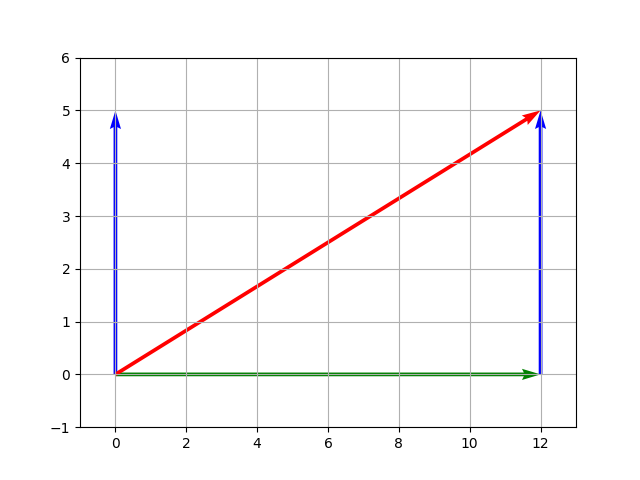
\includegraphics[width=100mm, scale=0.8]{vector_diagram.png}
In the figure, blue arrow with its tail at origin represents $\vec{a}$, which can also be displaced to have its tail at the coordinate (12,0) to complete the triangle.\\
The red arrow represents $\vec{a}+\vec{b}$ (by Triangle Law of Vector Addition) and green arrow represents $\vec{b}$. Vectors $\vec{a}$ and $\vec{b}$ are perpendicular, $\left| \vec{a} \right| = 5$ and $\left| \vec{a}+\vec{b} \right| = 13$, hence by the diagram, $\left| \vec{b} \right|$ should be 12 since by Baudhāyana Sulbasūtra, 5, 12, and 13 form a triplet which is quite famous ($5^2+12^2=13^2$)
\end{document}
